\section{Constant stretch transformations}\label{chapter:constant_stretch}

\fda{edit this section as discussed in the meeting}
\subsection{Some preliminaries}

Consider two nodes \(v,\ w \in V\). 
Let the \emph{infinity norm} be defined as \(L_\infty = \linfty{v - w} \coloneqq \max\parens{\abs{v_x - w_x},\ \abs{v_y - w_y}}\). 
Let \(d \coloneqq \max_{r \in R}\parens{\linfty{\iconf{s}{r} - \iconf{t}{r}}}\). 
Note that \(\linfty{v - w} \leq \manhattan{v - w} \leq 2\cdot \linfty{v - w}\).

\subsection{Transformations by disjoint swap routines}

Given a \(2 \times 3\) (or \(3 \times 2\)) rectangle with up to six robots, \cite{siamcomp/DemaineFKMS19} shows that any two configurations \(\conf{1}\) and \(\conf{2}\) of this rectangle are within 7 transformation steps from each other. 
This results in a workspace being able to be subdivided into multiple of these rectangular blocks that can be permuted independently in constant time.
See \cref{fig:swap3} for a visual of swapping two neighboring robots.

\begin{figure}[h]
	\centering
	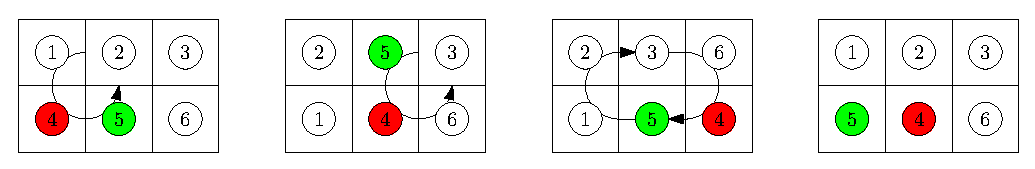
\includegraphics[width=0.8\linewidth]{ipe/swap_ex.eps}
	\caption{
		Swapping two robots in three steps using a fixed amount of space.
	}\label{fig:swap3}
\end{figure}

\cite{algorithmica/MarbergG88} introduced an algorithm called \emph{Rotatesort} which can sort an discrete \(n_1 \times n_2\) grid of \emph{elements} in parallel in \(\mathcal{O}(n_1 + n_2)\) time.
Rotatesort is not built with robots in mind, and uses only swap operations: swapping the positions of two adjacent elements.
We consider two swaps to be disjoint when their four associated positions are distinct.
At any timestep, Rotatesort requires that we can execute any disjoint swap operations in parallel.

These operations obviously break the non-swapping constraint in \cref{req:no_swaps} of our robot motion planning problem, however, as seen in \cref{fig:swap3}, we can clearly simulate an atomic swap operation in \(\mathcal{O}(1)\) time for any single swap.
This can be done in parallel for swaps in disjoint \(2 \times 3\) rectangles, and by repeatedly overlapping the rectangles in different patterns for \(\mathcal{O}(1)\) times we can simulate any single transformation step that disregards the non-swapping constraint in constant time.

As \(\mathcal{O}((n_1 + n_2) \cdot \mathcal{O}(1)) = \mathcal{O}(n_1 + n_2)\), this implies that for an \(n_1 \times n_2\) workspace there is an efficient algorithm that can always compute a schedule with \(\mathcal{O}(n_1 + n_2)\) makespan. 
This clearly works even for workspaces with densities of up to 100\%, i.e.~no free vertices available.

% As longer distances would ideally be traversed monotonously moving in the same direction, and not back and forth, continuously transforming \(n_1 \times n_2\) rectangles, \cite{siamcomp/DemaineFKMS19} comes up with the idea of combining Rotatesort with so-called \emph{subflows}. 

\subsection{Utilizing subflows to achieve constant stretch}

Building upon the previous findings, \cite{siamcomp/DemaineFKMS19} further details an algorithm for achieving a \emph{constant stretch factor} for arbitrary start and target configurations.
By subdividing the workspace into fairly large but \(\mathcal{O}(d)\) sized tiles, any transformations that is within such a tile can be done in linear time w.r.t.~the maximum horizontal or vertical distance, using the previous findings.
They show that \(\mathcal{O}(d)\) non-intersecting \emph{subflows} can be used to swap robots between tiles efficiently, using \(\mathcal{O}(d)\) transformation steps.
The improvement in makespan essentially comes from putting robots in queues, and then constantly moving them in the same direction, in contrast with constantly swapping adjacent robots like in the schedules computed by Rotatesort.

Preprocessing the tiles to be compatible with non-intersecting subflows means swapping some robots between tiles. 
Otherwise, diagonally neighboring tiles would have robots going both ways, crossing paths. 
\cite{siamcomp/DemaineFKMS19} shows that this preprocessing is possible to do in \(\mathcal{O}(d)\) steps. 

As a result, on a very high level, the following algorithm allows for a constant stretch schedule for any arbitrary workspaces with up to 100\% densities: 
\begin{enumerate}
	\item Preprocess for non-intersecting subflows in \(\mathcal{O}(d)\) steps
	\item Move all robots to their respective target tiles using subflows in \(\mathcal{O}(d)\) time
	\item All robots are now in their target tiles. Transform all tiles to their target configurations in parallel in \(\mathcal{O}(d)\) steps
\end{enumerate}

The schedule for this can be computed in \(\mathcal{O}(dn_1 n_2)\) time \cite{siamcomp/DemaineFKMS19}, and it can clearly be executed in \(\mathcal{O}(d)\) time. 
\(\mathcal{O}(d)\) is equivalent to a constant stretch factor, which also implies a constant approximation factor. 

